\section{Serial and parallel algorithms performance} \label{s:results:performance-serial-parallel}

\begin{figure}[!htbp]
	\centering
	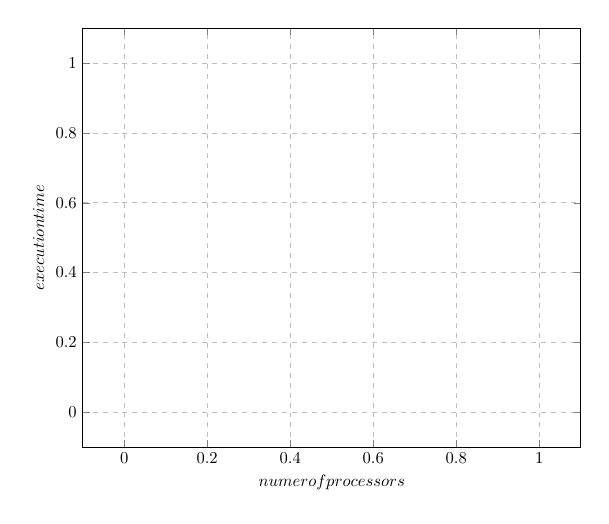
\begin{tikzpicture}[scale=0.6]	 	
	\pgfplotsset{width=\textwidth}
		\begin{axis}[
			xlabel = {$numer of processors$},
			ylabel = {$execution time$},
			%ymin = -1, ymax = 1,
			%xmin = 5, xmax = 13,
			%minor y tick num = 1,
			ymajorgrids=true,
			xmajorgrids=true,
			grid style=dashed,
			legend pos=north east
			]
			\addcustomplot{others/performance/crank-nicolson-parallel-final.csv}{red}{1}{CN}
			\addcustomplot{others/performance/implicit-upwind-parallel-final.csv}{green}{2}{IU}
			\addcustomplot{others/performance/explicit-upwind-parallel-final.csv}{blue}{2}{EU}
		\end{axis}
	\end{tikzpicture}
	\caption{Numerical solution comparison using implicit upwind scheme for serial and parallel algorithms. $\gls{CFL} = 0.01$ and $10000$ grid points.}
	\label{fig:comparison:implicit-upwind}
\end{figure}